\section{Results}

\subsection{Domain-shift}\label{sec:domain}
%\textbf{Given that Multi30K and COCO are both collections of crowdsourced literal descriptions of images, how well does a model trained on one dataset perform on the other? Vinyals reports that there is a domain-shift problem for captioning (CVPR 2015).}


\paragraph{Stuff}
In all our experiments the target domain is the M30K data set and add extra
English monolingual data in from COCO. Both collections of crowd-sourced 
literal descriptions of images and we expect a considerable overlap between
domains. First we quantitatively assess the distance between the 
M30K and COCO domains and if using the COCO data set can improve
performance in the M30K domain. We train three English image-sentence 
ranking models, 
one on M30K, the second on 
COCO and the third on both. In all cases we report results on 
the test portion of the English M30k in Figure~\ref{fig:domain}. 
The results show that there is considerable 
difference between the domains and training on 
COCO results in much lower test performance on the M30K. 
However, the domains also overlap 
between the domains as shown by the much higher than 
random R@10 scores for the COCO-only experiment, and by the 
performance boost when training on both the M30K and COCO data sets jointly.\\

\begin{figure}
    \centering
    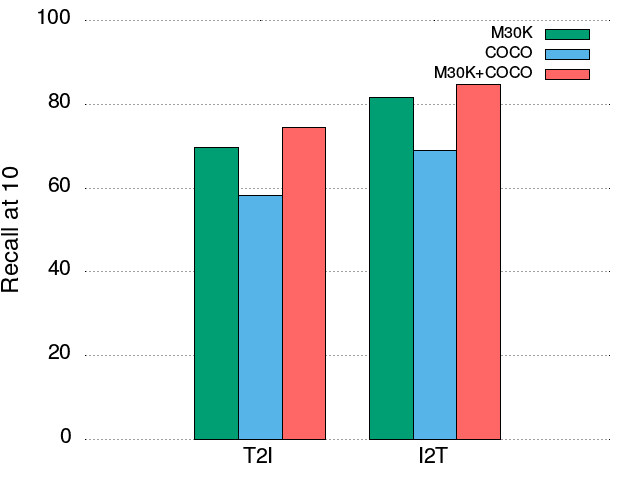
\includegraphics[scale=0.4]{assets/drift.png}
    \caption{Seed 409, early stopping done and R@10 reported on the dev set of the M30K datasets.}
    \label{fig:domain} 
\end{figure}

\subsection{Training with disjoint datasets}
\textbf{Set the baselines for training over disjoint datasets. No distant supervision version. Just the disjoint data.}

\paragraph{The findings}
Results on English Table~\ref{tab:English}:
\begin{enumerate}
    \item Line 1. vs. Line 4.: COCO improves M30K English.
    \item Line 2. vs. Line 4.: Adding more monolingual improves much more than
    adding German.
    \item Line 5. vs. Line 6.: Caption--caption loss further improves of course.
\end{enumerate}

Results on German Table~\ref{tab:German}:
\begin{enumerate}
    \item Line 1. vs. Line 4.: COCO improves M30K German.
    \item Line 2. vs. Line 4.: Adding the large English disjoint data set COCO 
    improves less than the aligned German.
    \item Line 3. vs. Line 2. and Line 5.: Adding both aligned and disjoint 
    together.
    \item Line 5. vs. Line 6.: The caption--caption loss further improves.
\end{enumerate}

In Section~\ref{sec:domain} we observe a considerable difference between the 
M30K domain, however, using COCO as an additional data source does improve 
performance on the target English M30K test set. In the following experiments
we assess whether the German M30K results can also be improved by the disjoint
COCO English set.

\begin{comment}
\begin{table}
    \centering
    \renewcommand{\arraystretch}{1.3}
    \begin{tabular}{ccccccc}
        \toprule
        c2c &    De         & En         & COCO       & I $\rightarrow$ T & T $\rightarrow$ I\\
        \midrule
        & \checkmark &            &            & 74.0              & 60.8 \\
        & \checkmark & \checkmark &            & 75.9              & 62.8  \\
        \checkmark & \checkmark &\checkmark &  &    77.4 & 64.7   \\ 
        & \checkmark &            & \checkmark & 75.4              & 61.5\\
        %2 &\checkmark & \checkmark  &  &  77.4 & 63.0  &  83.3 &  72.2 \\
        %4 & \checkmark &\checkmark & \checkmark  &  \checkmark &  78.0 & 65.4  &  82.3 &  72.6 \\
        \bottomrule
    \end{tabular}
    \caption{German results trained in monolingual, aligned, and disjoint settings.}
    \label{tab:addcoco}
\end{table}
\end{comment}

\paragraph{Disjoint German English model}

We train a disjoint model
using the German data from M30K, but COCO as the English
resource. We report the results in Table~\ref{tab:addcoco}.
Lines 2, 3 show that adding the M30K image-aligned English sentences to the
German training data the results are improved and further improvements can be
obtained by running the caption--caption objective. This finding reproduces 
that of \cite{kadar2018conll}. The German M30K model is also 
improved when adding the disjoint COCO as demonstrated in line 4., however, 
notice that the improvement is much smaller especially on T $\rightarrow$ I. 
This result contradicts that  of \cite{kadar2018conll}, who observe
the same improvements from aligned or disjoint images. 
This difference in findings is most likely due to the fact that
\cite{kadar2018conll} creates a disjoint data set artificially
from M30K, while in our setup we have two truly disjoint sets.

\paragraph{Improving bilingual model with disjoint English}
Now let us examine whether adding the extra disjoint COCO data set to
the bilingual model trained on the aligned German-English M30K adds 
further performance improvements. 
For this we train a bilingual model on M30K with 
and without caption--caption loss and the same models with the
COCO dataset added.  The results for both experiments are reported in 
Table~\ref{tab:bilingaddcoco}. Adding COCO to the bilingual M30K 
model improves performance as shown by the difference between line 1. and
line 3. The overall best performance is achieved with training on all
three data sets and adding the caption--caption loss, however, the 
image-retrieval performance (I $\rightarrow$ T) is lower than without the 
c2c loss in this setting. 


\begin{comment}
\begin{table*}
    \centering
    \renewcommand{\arraystretch}{1.3}
    \begin{tabular}{cccccccc}
        \toprule
        \multicolumn{4}{c}{Sources} & \multicolumn{2}{c}{De} & \multicolumn{2}{c}{En} \\
        c2c & De & En   & COCO  & I $\rightarrow$ T &  T $\rightarrow$ I  & I $\rightarrow$ T &  T $\rightarrow$ I\\
        \midrule
         &\checkmark & \checkmark  &  &  75.9  & 62.8   & 80.5  & 68.8   \\ 
         \checkmark &\checkmark & \checkmark  &  &  77.4 & 64.7   & 81.1  & 70.8   \\ 

         &\checkmark & \checkmark  &  \checkmark &  77.4 & 63.0  &  83.3 &  72.2 \\
       \checkmark &\checkmark & \checkmark  &  \checkmark &  78.0 & 65.4  &  82.3 &  72.6 \\
        \bottomrule
    \end{tabular}
    \caption{Improving bilingual model with disjoint English}
    \label{tab:bilingaddcoco}
\end{table*}
\end{comment}


\begin{comment}
\begin{table*}
    \centering
    \renewcommand{\arraystretch}{1.3}
    \begin{tabular}{c|c|ccc|cccc}
        \toprule
        & C2C & \multicolumn{3}{c}{Sources} & \multicolumn{2}{c}{De} & \multicolumn{2}{c}{En} \\
        & & De & En   & COCO  & I $\rightarrow$ T &  T $\rightarrow$ I  & I $\rightarrow$ T &  T $\rightarrow$ I\\
        \midrule
        1 & &\checkmark & \checkmark  &  &  75.9  & 62.8   & 80.5  & 68.8   \\ 
        2 & &\checkmark & \checkmark  &  \checkmark &  77.4 & 63.0  &  83.3 &  72.2 \\
        3 & \checkmark &\checkmark & \checkmark  &  &  77.4 & 64.7   & 81.1  & 70.8   \\ 

      4 & \checkmark &\checkmark & \checkmark  &  \checkmark &  78.0 & 65.4  &  82.3 &  72.6 \\
        \midrule
        5 &  & \checkmark &  &  & 74.0  & 60.8   &  &\\
        6 &  &\checkmark &   & \checkmark     & 75.4 & 61.5  &  &\\
        \bottomrule
    \end{tabular}
    \caption{kk}
    \label{tab:addcoco}
\end{table*}
\end{comment}


\subsection{Distant supervision by translation}

Results on German Table~\ref{tab:German}:

\begin{enumerate}
    \item Line 7. vs. Line 1.: Adding the German translated COCO improves over 
    German monolingual.
    \item Line 7. vs. Line 2.: Adding the disjoint translated German COCO 
    provides more improvement than the English M30K.
    \item Line 7. vs. Line 4.: The translated German COCO improves much more than
    the original English.
    \item Line 8. vs. Line 7.: Adding both the English and translated COCO adds
    further improvement, even though the English-German COCO are just translations
    of each other.
    \item Line 9. vs. Line 8.: Adding the M30K English on top of the German COCO is
    better than adding the original English version of COCO.
    \item Line 10 vs. Line 9.:  Caption--caption makes it worse?????
    \item Line 11. vs. Line 7. Line 8. and Line 9.: Adding the aligned English 
    together with both the German and original English is better than any of
    the combination of these.
    \item Line 12.: Adding the caption--caption on top of all data sets is the best.
\end{enumerate}


Results on English Table~\ref{tab:English}:

\begin{enumerate}
    \item Line 7. vs. Line 1.: Adding the German translated COCO improves over 
    only training on English M30K.
    \item Line 8. vs. Line 3.: Adding the disjoint translated German COCO 
    provides slightly less improvement than more improvement than 
    the aligned German M30K.
    \item Line 9. vs. Line 5.: Having both the English and German COCO is 
    considerably worse than only having the COCO English.
    \item Line 10. vs. Line 3.: Adding the German translated COCO on top of the
    bilingual M30K model improves performance.
    \item Line 11. vs. Line 10.: The caption--caption here improves.
    \item Line 11. vs. Line 10. and Line 9.: Adding the original English COCO
    on top of the translated German COCO and the M30K German imrpoves performance,
    however, it is still slightly lower than just adding English COCO on top of
    the English M30K.
    \item Line 13. Best results are achieved with all the data sets witht 
    caption--caption loss. 
\end{enumerate}

Here we add additional German training data by translating the original English
COCO captions to German using a pre-trained OpenNMT model.

\begin{comment}
\begin{table}
\setlength{\tabcolsep}{5pt}
    \centering
    \begin{tabular}{cccccc}
         \toprule
         De         & COCO        & OpenNMT      & c2c        & I $\rightarrow$ T & T $\rightarrow$ I  \\
         \midrule
         \checkmark & \checkmark  &              &            & 75.4              & 61.5 \\
         \checkmark &             & \checkmark   &            & 77.1              & 63.7 \\               
         \checkmark & \checkmark  & \checkmark   &            & 77.8              & 63.9 \\
         \checkmark & \checkmark  & \checkmark   & \checkmark &                   &  \\
         \bottomrule
    \end{tabular}
    \caption{Improving German with COCO plus OpenNMT}
    \label{tab:opennmt}
\end{table}
\end{comment}

\begin{comment}
\begin{table*}
    \centering
    \renewcommand{\arraystretch}{1.3}
    \begin{tabular}{cccccccccc}
        \toprule
        \multicolumn{4}{c}{Sources} & & \multicolumn{2}{c}{De} & \multicolumn{2}{c}{En} \\
        c2c & De & En   & COCO & OpenNMT & I $\rightarrow$ T &  T $\rightarrow$ I  & I $\rightarrow$ T &  T $\rightarrow$ I & rsum\\
        \midrule
         &\checkmark & \checkmark  & \checkmark &  & 77.4 & 63.0  &  \textbf{83.3} &  72.2 & 694.6  \\ 
         \checkmark &\checkmark & \checkmark  & \checkmark &  &  78.0 & 65.4  &  82.3 &  72.6 & 702.9  \\ 
       & \checkmark & \checkmark  &  \checkmark & \checkmark &  \textbf{79.8} & 65.2 & 82.6 & 71.6 & 702.9 \\
\checkmark & \checkmark & \checkmark  &  \checkmark & \checkmark & 79.1 & \textbf{67.7} & 82.4 & \textbf{73.2} & 717.0 \\

        \bottomrule
    \end{tabular}
    \caption{Improving bilingual model with OpenNMT}
    \label{tab:bilingopennmt}
\end{table*}
\end{comment}
\paragraph{Disjoint German English model}

In Table~\ref{tab:opennmt} we report the results for the case of improving the
German model with the disjoint COCO data set. Adding the extra translated 
German COCO data set considerably improves the performance compared to adding
the English sentences. The result suggests that the model can better exploit 
more monolingual training data with sufficient translation quality than
natural English sentences. Adding the original English COCO sentences
on top of the translated German captions (line 3.) provides only 
slightly very slight gains. 

\begin{comment}

LINE3 WITHOUT START UP
m30ken
Rsum: 366.857330703
Image to text: R@1 45.3 | R@5 72.9 | R@10 82.6 | Medr 2.0 | Meanr 11.3 | Average 67.0
Text to image: R@1 33.0 | R@5 61.4 | R@10 71.6 | Medr 3.0 | Meanr 23.1 | Average 55.3
m30kde
Rsum: 336.127547666
Image to text: R@1 40.0 | R@5 68.9 | R@10 79.8 | Medr 2.0 | Meanr 15.8 | Average 62.9
Text to image: R@1 27.5 | R@5 54.7 | R@10 65.2 | Medr 4.0 | Meanr 34.9 | Average 49.2

LINE4 WITHOUT START UP
m30ken
Rsum: 373.576594346
Ima ge to text: R@1 45.9 | R@5 73.7 | R@10 82.4 | Medr 2.0 | Meanr 11.7 | Average 67.3
Text to image: R@1 35.1 | R@5 63.3 | R@10 73.2 | Medr 3.0 | Meanr 21.6 | Average 57.2
m30kde
Rsum: 343.425378041
Image to text: R@1 41.0 | R@5 69.4 | R@10 79.1 | Medr 2.0 | Meanr 15.9 | Average 63.1
Text to image: R@1 29.4 | R@5 56.9 | R@10 67.7 | Medr 4.0 | Meanr 31.0 | Average 51.3

\end{comment}


\paragraph{Improving bilingual model with disjoint English}
Here we train our baseline with the bilingual German-English M30K and add the
additional translated German-COCO captions on top. Results are reported in
Table~\ref{tab:bilingaddcoco}. Adding the extra German captions improves 
performance overall as shown in the difference between line 1. and line 3.
The overall best results are achieved when using all the data sets with the
caption--caption loss on both English-German M30K and COCO pairs. 


\begin{table*}[]
    \centering
    \renewcommand{\arraystretch}{1.0}
    \begin{tabular}{c|cccccc|cccccc}
        \hline
            &&&&&&& \multicolumn{3}{c}{I $\rightarrow$ T} & \multicolumn{3}{c}{T $\rightarrow$ I} \\
         & \rotatebox{90}{De} & \rotatebox{90}{En} & \rotatebox{90}{COCO} & 
         \rotatebox{90}{OpenNMT-De} & \rotatebox{90}{Pseudo-De} & \rotatebox{90}{c2c}  & R@1 & R@5 & R@10 & R@1 & R@5 & R@10 \\
         \hline
         & \multicolumn{11}{l}{\textit{In-domain Multi30K}} \\
         \hline
         1 &  \checkmark  & & & & & & 34.9 & 64.1  & 76.2  & 24.6 & 50.1 & 61.3 \\
         2 & \checkmark & \checkmark & & & &  & \textbf{38.6}  & 66.9  &  77.9 & 26.0 & 52.2  & 63.0\\
         3 & \checkmark & \checkmark &  & & & \checkmark & 38.3 & \textbf{68.3} & \textbf{78.8} & \textbf{27.7} & \textbf{54.9} & \textbf{66.0}  \\
         \hline
         & \multicolumn{11}{l}{\textit{In-domain and out-of-domain COCO}} \\
         \hline
         4 & \checkmark & & \checkmark & &  &  & 36.4 & 65.9  & 77.6 & 25.7  & 51.6 & 62.6 \\
         5 & \checkmark & \checkmark & \checkmark & & & & 39.2  & 67.8  & 79.1 & 27.1 & 53.2  &  64.0  \\
         6 & \checkmark & \checkmark & \checkmark & & & \checkmark  & \textbf{40.6} & \textbf{70.5}  & \textbf{81.1}  & \textbf{28.8} & \textbf{56.3}  & \textbf{67.3} \\
         \hline
         & \multicolumn{11}{l}{\textit{In-domain and distant supervision: translation}} \\
         \hline
         7 & \checkmark & &  & \checkmark & & & 38.5 & 68.4 & 79.6 & 26.6 & 53.7 & 64.4\\
         8 & \checkmark & & \checkmark  & \checkmark & & & 39.1 & 69.8 & 80.2 & 27.5 & 54.2 & 64.7 \\
         9 & \checkmark & \checkmark &  & \checkmark & & & 39.8 & 69.6 & 81.0 & 27.6 & 54.8 & 65.5 \\
         10 & \checkmark & \checkmark &  & \checkmark & & \checkmark & 38.2 & 66.3 & 77.0 & 27.2 & 54.2 & 65.5 \\
         11 & \checkmark & \checkmark & \checkmark  & \checkmark & & & 40.2 & 71.2 & 81.9 & 28.3 & 55.6 & 66.1 \\
         12 & \checkmark & \checkmark & \checkmark  & \checkmark & & \checkmark & \textbf{43.5} & \textbf{73.3} & \textbf{82.5} & \textbf{30.5} & \textbf{58.8} & \textbf{69.3} \\

         \hline
         & \multicolumn{11}{l}{\textit{Distant supervision: psuedopairs}} \\
          \hline
         13 &\checkmark & & \checkmark  &  & \checkmark & & 36.7 &  65.1  & 76.3  & 25.2  & 51.3 &   62.2\\
         13 &\checkmark & & \checkmark  &  & 25\% & & 36.6 &  65.2  & 76.8  & 25.0  & 51.6 &   62.9\\
         13 &\checkmark & & \checkmark  &  & 75\% & & 36.7 &  63.8  & 75.8   & 24.6  & 51.1 &   62.1\\
         \hdashline
         14 & \checkmark & & \checkmark  &  & \checkmark & \checkmark  & 35.6  & 65.3 & 75.6  & 25.0  &  51.2 & 62.4 \\
         14 & \checkmark & & \checkmark  &  & 25\% & \checkmark  & 33.6  & 63.5 & 75.6 & 23.9 &  50.3 & 61.5 \\
         14 & \checkmark & & \checkmark  &  & 75\% & \checkmark  &  &  &  &  &  & \\
         \hdashline
         15 & \checkmark & \checkmark & \checkmark  &  & \checkmark &  & 37.9  &  68.3  & 78.8 &  26.8 & 53.9 & 64.6 \\
        15 & \checkmark & \checkmark & \checkmark  &  & 25\% &  &  38.4 & 68.9 & 78.9 &  26.8 & 53.3 & 64.4  \\
         15 & \checkmark & \checkmark & \checkmark  &  & 75\% &  & 37.7 & 66.8 & 78.7 & 26.2  & 53.1 & 63.6 \\
         \hdashline
         16 & \checkmark & \checkmark & \checkmark  &  & \checkmark & \checkmark  & 39.9 & 69.9  & 80.2 & 29.6 &  57.3 &  67.8 \\
         16 & \checkmark & \checkmark & \checkmark  &  & 25\% & \checkmark  & 41.5 & 70.4 & 80.8  & 28.9  & 56.8  & 67.2\\
         16 & \checkmark & \checkmark & \checkmark  &  & 75\% & \checkmark  & 40.3  &  69.3 &    79.1  &  27.9 & 55.6 & 66.8\\
    \end{tabular}
    \caption{Results reported on German}
    \label{tab:German}
\end{table*}



\begin{table*}[]
    \centering
    \renewcommand{\arraystretch}{1.0}
    \begin{tabular}{c|cccccc|cccccc}
        \hline
            &&&&&& \multicolumn{3}{c}{I $\rightarrow$ T} & \multicolumn{3}{c}{T $\rightarrow$ I} \\
         & \rotatebox{90}{De} & \rotatebox{90}{En} & \rotatebox{90}{COCO} & 
         \rotatebox{90}{OpenNMT-De} & \rotatebox{90}{Pseudo-De} & \rotatebox{90}{c2c}  & R@1 & R@5 & R@10 & R@1 & R@5 & R@10 \\
         \hline
         & \multicolumn{11}{l}{\textit{In-domain Multi30K}} \\
         \hline
         1 &  & \checkmark & & & &  & 40.5  &  69.6  &  79.9   & 28.8 & 58.3 & 69.4  \\
         2 &  &  & \checkmark & & & & 34.4  & 61.4  &  72.1 & 24.8 & 50.3  & 61.1\\
         3 & \checkmark & \checkmark & & & &   & 41.4 & 70.9 & 81.0 & 29.9 & 59.6 & 70.0 \\
         4 & \checkmark & \checkmark &  & & & \checkmark & \textbf{42.8} & \textbf{72.0} & \textbf{81.2}  & \textbf{32.1} & \textbf{61.4} & 
          \textbf{72.2} \\
         \hline
         & \multicolumn{11}{l}{\textit{In-domain + out-of-domain COCO}} \\
         \hline
         5 & & \checkmark & \checkmark & &  &  & 46.2 & 75.6 & 83.6 & 33.4 & 62.5  & 73.1  \\
         6 & \checkmark & \checkmark & \checkmark & & &  & 46.0  & 75.3 & 83.9  &33.6 & 62.7 &  73.3  \\
         7 & \checkmark & \checkmark & \checkmark & & & \checkmark  & \textbf{46.5} & \textbf{75.2} & \textbf{83.8} & \textbf{34.8} & \textbf{64.4}  & \textbf{74.3} \\
         \hline
         & \multicolumn{11}{l}{\textit{Distant supervision: translation}} \\
         \hline
         8 & & \checkmark &  & \checkmark & & & 42.2 & 71.1 & 80.6 & 30.5 & 57.8 & 68.7 \\
         9 & & \checkmark & \checkmark  & \checkmark & & & 45.6 & 72.9 & 81.1 & 33.0 & 61.0 & 71.8  \\
         10 & \checkmark & \checkmark &  & \checkmark & & & 43.8 & 72.0 & 81.4 & 30.9 & 60.1 & 70.9 \\
         11 & \checkmark & \checkmark &  & \checkmark & & \checkmark & 44.9 & 73.2 & 82.1 & 33.8 & 61.7 & 72.2 \\
         12 & \checkmark & \checkmark & \checkmark  & \checkmark & & & 46.8 & 74.7 & 83.4 & 33.6 & 62.9 & 73.2 \\
         13 & \checkmark & \checkmark & \checkmark  & \checkmark & & \checkmark & \textbf{47.5} & \textbf{75.7} & \textbf{84.1} & \textbf{36.2} & \textbf{65.6} & \textbf{75.6} \\

         \hline
         \multicolumn{12}{l}{\textit{Distant supervision: psuedopairs}} \\
         \hline
         14 & \checkmark & \checkmark & \checkmark  &  & \checkmark &  & 46.4  & 75.4  & 83.2  &  33.3 & 62.5 & 73.1\\
         15 & \checkmark & \checkmark & \checkmark  &  & 25\% &  & 46.9  & 74.9  & 83.4   &  33.7 & 62.8 & 73.1\\
        17 & \checkmark & \checkmark & \checkmark  &  & 75\% &  & 46.1  & 75.1 & 83.7  &  33.5  & 62.9  & 73.3 \\
        \hdashline
         18 & \checkmark & \checkmark & \checkmark  &  & \checkmark & \checkmark  &  47.7 & 75.3   &   83.7 & 35.3 & 65.1 & 75.2 \\
        19 & \checkmark & \checkmark & \checkmark  &  & 25\% & \checkmark  & 47.5  & 75.3 & 83.8 & 34.9  & 64.2 &  74.4 \\
        20 & \checkmark & \checkmark & \checkmark  &  & 75\% & \checkmark  & 45.9 & 73.5  & 82.6  & 34.0 & 63.6 & 74.0  \\
    \end{tabular}
    \caption{Results reported on English}
    \label{tab:English}
\end{table*}

\begin{comment}

\begin{table*}
    \centering
    \begin{tabular}{cccccccc}
         \toprule
           & \multicolumn{2}{c}{Multi30K} & \multicolumn{2}{c}{COCO}      & c2c\\
         V & De           & En            & OpenNMT          & En         & loss       & I $\rightarrow$ T & T $\rightarrow$ I  \\
         \midrule
         10K & \checkmark &               &                  &            &            & 74.9              & 60.6 \\
         18K & \checkmark & \checkmark    &                  &            &            & 75.9              & 62.8 \\
         18K & \checkmark & \checkmark    &                  &            & \checkmark & 77.4              & 63.0 \\
         ??? & \checkmark & \checkmark    &                  & \checkmark & \checkmark & 78.2              & 65.4 \\
         ??? & \checkmark &               &                  & \checkmark &            & 75.4              & 61.5 \\
         \midrule
         24K & \checkmark &               & \checkmark       &            &            & 77.1              & 63.7 \\               
         32K & \checkmark &               & \checkmark       & \checkmark &            & 77.8              & 63.9 \\
         34K & \checkmark & \checkmark    & \checkmark       & \checkmark &            & 79.8              & 65.2 \\
         34K & \checkmark & \checkmark    & \checkmark       & \checkmark & \checkmark & 79.6              & 67.3\\
         \midrule
    \end{tabular}
    \caption{Performance of training a German model with OpenNMT translated COCO sentences. No caption--caption loss. Early-stopping on DE M30K. V: Number of words in the model vocabulary. The top lines show the performance of models trained on only human-annotated data. The bottom lines show the performance of models train on extra automatically annotated data. NB: None of the c2c models were trained with Akos' warm-up trick.}
    \label{tab:opennmt}
\end{table*}
\end{comment}


\paragraph{Improving bilingual model with disjoint English}

%We try to estimate the utility of training with automatically translated German sentences for the COCO dataset. The COCO sentences were translated with an off-the-shelf OpenNMT English-German translation model. The results can be seen in Table \ref{tab:opennmt}. Line 2: It helps to co-train with the English M30K data (already known). Line 3: It helps to co-train with English COCO (already known) but not as much as co-training with the English M30K. This is probably due to the benefit of training on in-domain data. Line 6: It helps even more to train with OpenNMT-translated COCO sentences compared to English COCO sentences. This is likely because we are updating the German word representations with the German out-of-domain data. Line 7: It helps a litte bit more if we co-train with English COCO and OpenNMT-translated COCO. Line 8: Large improvement if we co-train with all the data (English Multi30K, English COCO, and OpenNMT-translated COCO). Line 9: Large improvement in T$\rightarrow$I performance if we include the c2c loss. Q: Why do the improvements saturate as we add more data? Confound: our model contains many more learnable embeddings with both languages and the translated German data. More likely explanation: we're spending too many updates fitting the out-of-domain data (compare Line 7 and Line 8).


\subsection{Distant supervision with pseudo-pairs}

\paragraph{Disjoint German English model}
Here we first train the disjoint model with the German captions from M30K
and the English sentence from COCO. Then we use this model to create the 
new pseudo-pairs based on sentence similarity. Given the new data set the
model is re-trained using all three data sets below the findings with  
line numbers in Table 1.:

\begin{enumerate}
    \item 7 vs. 13: Pseudo-pairs degrade performance.
    \item Removing the bottom 25\% makes it a bit better.
    \item Keeping only the top 25\% makes it worse.
\end{enumerate}

Overall pseudo-pairs didn't work.

\subsection{All the stuff in Table~\ref{tab:aligned}}

Each element in the enumeration describes the corresponding line in Table~\ref{tab:aligned}. All models are trained with max-violation loss
function. For models trained with multiple data sets we sample from each
data set with uniform probability. When we train with both image--caption
and caption--caption loss we decide with a fair coin flip which task to
perform and from that task the data set is sampled with uniform
probability. As observed already in the VSE++ paper the max-violation 
loss has this property that it has a slow start-up period. In our
experiments the max-violation loss oscillates around the value
$$\textrm{batch-size} \times \alpha \times 2$$. When only training the
caption--caption loss we observed that it pushes all sentences to have
cosine similary of 1.0 and the training gets stuck and that starting 
training with both image--caption and caption--caption loss does not 
converge. To solve the issue we start training with the image--caption 
objective only and add the caption--caption loss after the 
"start-up time" when the the loss is  smaller than $(\textrm{batch-size} \times \alpha \times 2)-2.0$


\begin{enumerate}
    \item German monolingual 
    \item English monolingual
    \item Model trained on English and German M30K with early stopping on
    the sum of scores from the validation set of  English and German
    M30K.
    \item Same as line 2., but COCO data set added to the 
    training.
    \item Model trained on the same data sets as the line 4. with the
    the synthetic data set created with the model from line 4. added
    to the set of traning sets.
    \item Same as line 3. with the added caption--caption loss.
    \item Same as line 4. with the added caption--caption loss.
    \item Trained on M30K English + German and the COCO data set plus
    the synthetic data set generated by the model in line 8. This model
    is trained \textbf{without} the caption--caption loss.
    \item Same as line 9., but with the caption--caption loss. In this
    case the c2c objective is trained with the English-German sentence 
    pairs from M30K and also the synthetically generated true English
    COCO captions and their pseudo-pairs in German. (one of the seeds is
    completely terrible, the other 2 are pretty good)
\end{enumerate}

\subsection{Experiment 1.}

\begin{comment}
\begin{table*}
    \centering
    \renewcommand{\arraystretch}{1.3}
    \begin{tabular}{c|c|cccccccc}
        \toprule
        & C2C & \multicolumn{4}{c}{Sources} & \multicolumn{2}{c}{De} & \multicolumn{2}{c}{En} \\
        & & De & En   & COCO & De $\rightarrow$ COCO & I $\rightarrow$ T &  T $\rightarrow$ I  & I $\rightarrow$ T &  T $\rightarrow$ I\\
        \midrule
        %1 & &\checkmark & & & & 74.0 & 60.8  \\
        %2 & & & \checkmark  & & & & &  &  \\ 
        %\midrule
        3 & &\checkmark & \checkmark  &  & & 75.9  & 62.8   & 80.5  & 68.8   \\ 
        4 & &\checkmark & \checkmark  &  \checkmark & & 77.4 & 63.0  &  83.3 &  72.2 \\
        5 & &\checkmark & \checkmark  &  \checkmark & \checkmark  & 77.5  & 63.1  & 82.8 &  72.0 \\
        \midrule
        6 & \checkmark & \checkmark & \checkmark  &  & & 77.4 & 64.7   & 81.1 & 70.8    \\
        7 & \checkmark & \checkmark & \checkmark  &  \checkmark & & 78.2  & 65.4   &  82.4  &  72.6 \\
        8 & & \checkmark  &  \checkmark & \checkmark & \checkmark & 78.0  & 65.4  & 82.3  &  72.6 \\
        9 & \checkmark &    \checkmark & \checkmark  &  \checkmark & \checkmark  & 77.7   & 65.5   & 82.7  & 72.7 \\ 
        \midrule
        \multicolumn{10}{c}{Threshold 75\%} \\
        8 & & \checkmark  &  \checkmark & \checkmark & \checkmark &  &  & &   \\
        9 & \checkmark &    \checkmark & \checkmark  &  \checkmark & \checkmark  &  & &  &  \\
        \midrule
        \multicolumn{10}{c}{Threshold 25\%} \\

    \end{tabular}
    \caption{Results of Experiment 1. Line 3: training a bilingual model improves over training monolingual models. Line 4: training with out-of-domain English-captioned COCO images further improves both De and En ranking performance. Line 5: training with pseudo De-COCO pairs annotated from the De-Multi30K dataset does not further improve De or En ranking performance.}
    \label{tab:aligned}
\end{table*}
\end{comment}


In this section we report our first set of experiments asking the question if the larger disjoint English corpus can improve the bilingual model trained on a smaller aligned English-German corpus. Out of the two sets of experiments, this can be considered the most data rich setup. 
We train five models for which the results we report in Table~\ref{tab:aligned}. The column labels "De" and "En" stand for
M30K-German and M30K-English respectively, while "De $\rightarrow$ COCO" stands for the pseudo-corpus created by annotating COCO images
with German captions using the sentence-similarity approach. Comparing
line 3 with line 1-2 shows that the bilingual joint training improves
performance also in our experiments. Adding COCO improves both German
and English results on M30K as demonstrated by line 3. While the
pseudo-data set improves image-to-text retrieval results by a small
margin it is detrimental to text-to-image ranking in our experiments. This final result was found in the No filtering strategy.

\begin{comment}

\begin{table*}[]
    \centering
    \begin{tabular}{cccc|cccc}
          & & & & \multicolumn{2}{c}{Ger} & \multicolumn{2}{c}{Eng} \\
          Ger & Eng   & COCO & Ger $\rightarrow$ COCO & I $\rightarrow$ T &  T $\rightarrow$ I  & I $\rightarrow$ T &  T $\rightarrow$ I\\
          \checkmark & & & & 74.8  & 62.2  \\
            & \checkmark  & & & & & 82.0 & 70.5 \\ 
           \checkmark & \checkmark  &  & & 78.7  & 65.1  & 82.6  & 71.6    \\ 
            \checkmark & \checkmark  &  \checkmark & & 80.0 & 66.6  & 84.2 &  74.6 \\ 
              \checkmark & \checkmark  &  \checkmark & \checkmark  & 80.2 & 66.0  & 84.4 & 74.1 \\
    \hline
     \checkmark &   &  \checkmark &  & 78.0   & 64.7 &   & \\
     \checkmark &   &  \checkmark & \checkmark  & 77.3   &  64.3  &  &

    \end{tabular}
    \caption{Early-stopping and results reported on the German and English M30K.}
    \label{tab:my_label}
\end{table*}
\end{comment}


\subsection{Experiment 2.}
In this second set of experiments we consider the setting where the 
German and English data sets are completely disjoint. For German we use
the M30K data set and for English we use COCO. As shown in 
Table~\ref{tab:disjoint} the bilingual model
improves upon the monolingual German one, however, the improvement
is smaller then in the aligned case (in Table~\ref{tab:aligned}).
Furthermore, the pseudo-pairs generated by sentence-similarity seem
to be slightly detrimental to the results.

\begin{table}[]
\setlength{\tabcolsep}{5pt}
    \centering
    \begin{tabular}{cccc|cc}
    \toprule
        %\multicolumn{3}{c}{Sources} & \multicolumn{2}{c}{De} \\[1ex]
        c2c & Ger &  COCO & pseudo & I $\rightarrow$ T &  T $\rightarrow$ I  \\
        \midrule
        %& \checkmark & & & 74.0  & 60.8  \\
        & \checkmark &    \checkmark &  & 75.4 & 61.5 \\
        & \checkmark &    \checkmark & \checkmark  & 74.8   & 61.6 \\
        \checkmark & \checkmark &    \checkmark & \checkmark  & 73.5   & 61.3 \\
        \midrule
        & \multicolumn{3}{c|}{25\% percentile} & 74.4 & 61.6 \\
        & \multicolumn{3}{c|}{75\% percentile} & 74.6 & 60.2 \\
       \checkmark & \multicolumn{3}{c|}{25\% percentile} &  &  \\
       \checkmark & \multicolumn{3}{c|}{75\% percentile} &  &  \\
        \bottomrule
    \end{tabular}
    \caption{Early-stopping and results reported on the German M30K. LAST ROW WITH CAPTION TO CAPTION}
    \label{tab:depseudo}
\end{table}

%\begin{table}[]
%    \centering
%    \begin{tabular}{lcc}
%        & T $\rightarrow$ I & I $\rightarrow$ T \\
%        De & 62.8  & 77.5\\
%        En-De & 64.8 & 77.8  \\
%        En-De-COCO & 66.2 & 79.5  \\
%        En-De-SyhtnCOCO & 64.9 & 77.7 
%    \end{tabular}
%    \caption{Caption}
%    \label{tab:my_label}
%\end{table}

%\begin{table*}[]
%    \centering
%    \begin{tabular}{lcccc}
%    & \multicolumn{2}{c}{T $\rightarrow$ I} & \multicolumn{2}{c}{I $\rightarrow$ T} \\
%    & En & De & En & De \\
%    \hline
%    \multicolumn{5}{c}{Monolingual} \\
%    \hline
%    M30K En &  69.8 & & 81.6 & \\ 
%    M30K De & & & & \\
%    \hline
%    \multicolumn{5}{c}{Aligned} \\
%    \hline
%    M30K   & 72.1  & 64.9 & 83.7  & 79.1 \\
%    M30K EN + M30K DE + COCO EN & 74.0 & 66.3 & 85.6 & 78.5  \\
%    M30K EN + M30K DE + COCO EN + $\sim$COCO-DE & 74.4 & 66.4 & 85.7 & 80.8 \\
%    \hline
%    \multicolumn{5}{c}{Disjoint} \\
%    \hline
%    M30K DE + Full COCO & 64.5 & 64.3 & 75.6 & 77.3\\
%    M30K DE + Small COCO & 57.3 & 62.7 & 71.0 & 75.2\\
%    \end{tabular}
%    \caption{How can we improve German retrieval performance? Seed 409, early stopping done and R@10 reported on the dev set of M30K task 2.}
%    \label{tab:biling}
%\end{table*}

\begin{comment}

\subsection{Bilingual lexicon induction}
The translation retrieval experiments shows that our models find accurate
translations for full sentences. Even though the model was trained with 
sentence level objectives we also test how well the model finds word translations. We compare to the best reported results
\cite{hartmann2017limitations}. All approaches, but ours are based on 
finding images for source and target words through online image search.
\texttt{AvgMax} and \texttt{MaxMax} searches for the best candidate
translation by computing image-similarity scores on the retrieved images
using CNN features. \texttt{CnnMean} and \texttt{CnnMax} approaches \cite{kiela2015visual} aggregate 
images features on a per word either taking the componentwise mean or max. This is followed by ranking target words with cosine similarity.
Our approach is simply to use cosine similarty between the learned word-embeddings of the visually grounded sentence embedding models.

\begin{table}[]
    \centering
    \begin{tabular}{lccc}
                          & NN   & VB   & ADJ  \\
         \texttt{AvgMax}  & \textbf{0.64} & \textbf{0.18} & \textbf{0.23} \\
         \texttt{MaxMax}  & 0.50 & 0.14 & 0.19 \\
         \texttt{CnnMean} & 0.60 & 0.14 & 0.20 \\
         \texttt{CnnMax}  & 0.59 & 0.16 & 0.17 \\
         \hline 
         \emph{align} & 0.42 & 0.12 & 0.09 \\
         \emph{aligh} + c2c & 0.46 & \textbf{0.18} & 0.11 \\
    \end{tabular}
    \caption{Mean reciprocal rank. Bold denotes the highest values per evaluation subset.}
    \label{tab:my_label}
\end{table}
\end{comment}

